\subsection{Excercise OpenAPIDMCar}
This task introduces the OpenAPI specification of the DM-Car.
It starts by taking a look at the used language in the specification and the general structure.
After that, the swagger editor is introduced with its UI and functionalities.
Finally, the specification of the \texttt{getCar()} method is analyzed in detail.

\subsubsection*{Markup Language}
\autoref*{lst:openapi-spec} shows the generic structure of an OpenAPI specification.
This listing also can be found in the tasks sheet \cite{CM-T-DMC}.

The used language is YAML (YAML Ain't Markup Language).
An alternative is JSON (JavaScript Object Notation).
Yet, there are some advantages of YAML over JSON in this context.

YAML is a superset of JSON, which means that every JSON file is also a valid YAML file.
However, YAML is more readable and easier to write than JSON.
JSON requires a more complex syntax, which makes it more error-prone.
The specification only needs to be readable for humans, no machine needs to parse it.
Therefore, JSON is more suitable for data interchange, while YAML is more suitable for configuration files.

\begin{lstlisting}[
    float=h,
    style=kit-cm,
    caption={Generic OpenAPI Specification Structure},
    label={lst:openapi-spec},
]
openapi : 3.0.1
info :
    title : API Specification < Microservice Name >
    description : < Description >
    version : 1.0.0
tags :
paths :
components :
    schemas :
\end{lstlisting}

\subsubsection*{OpenAPI Sections}
An OpenAPI specification consists of three general sections, each of which is described in the following.
\paragraph*{Info}
The \texttt{info} section contains general information about the API.
This includes the title, a description, the version, host, licensing, and the developers' contact information.

\paragraph*{Paths}
The \texttt{paths} section contains the API endpoints.
Each path defines a certain URL and the HTTP methods that can be used on this URL.
For each method, the request and response parameters are defined.
This enables simple navigation through the API, as this part provides a map of the API's overall functionality.

\paragraph*{Components}
The \texttt{components} section contains reusable components.
This includes schemas, data models, headers, and security schemes.
Therefore, parts of the specification can be defined once and reused in multiple places.
This reduces the amount of code, makes the specification more readable and improves the overall documentation quality.

\subsubsection*{Swagger Editor}
A screenshot of the Swagger Editor UI is shown in \autoref{fig:ms_dmCar_swaggerEditorUI}.

The left side of the UI shows the code, in this case, the OpenAPI specification written in YAML.
The right side shows the rendered specification.
The top bar provides further functionalities that will be explained in the following.

\texttt{File} provides the functionalities to import and export the specification.
The file also can be downloaded.

\texttt{Edit} allows the user to clear the file or convert it into a JSON file.

\texttt{Insert} provides the functionalities to insert a new path, definition, or security scheme.
This allows the user to quickly create a new endpoint or data model without having to write the code manually.

\texttt{Generate Server} creates server code containing the defined endpoints, routes, parameters and models from the specification.
This code can be downloaded as a ZIP file and in different programming languages.
This provides a quick way to create a basic server that can be extended with the actual functionality.

\texttt{Generate Client} generates client code.
This code uses the defined endpoints and models to send requests to the API, handling the request and response parameters.
The code can be downloaded as a ZIP file and in different programming languages.
This allows easy integration of the API into other applications.

\texttt{About} provides information and documentation about the Swagger Editor and access to the GitHub repository.

\begin{figure}
    \centering
    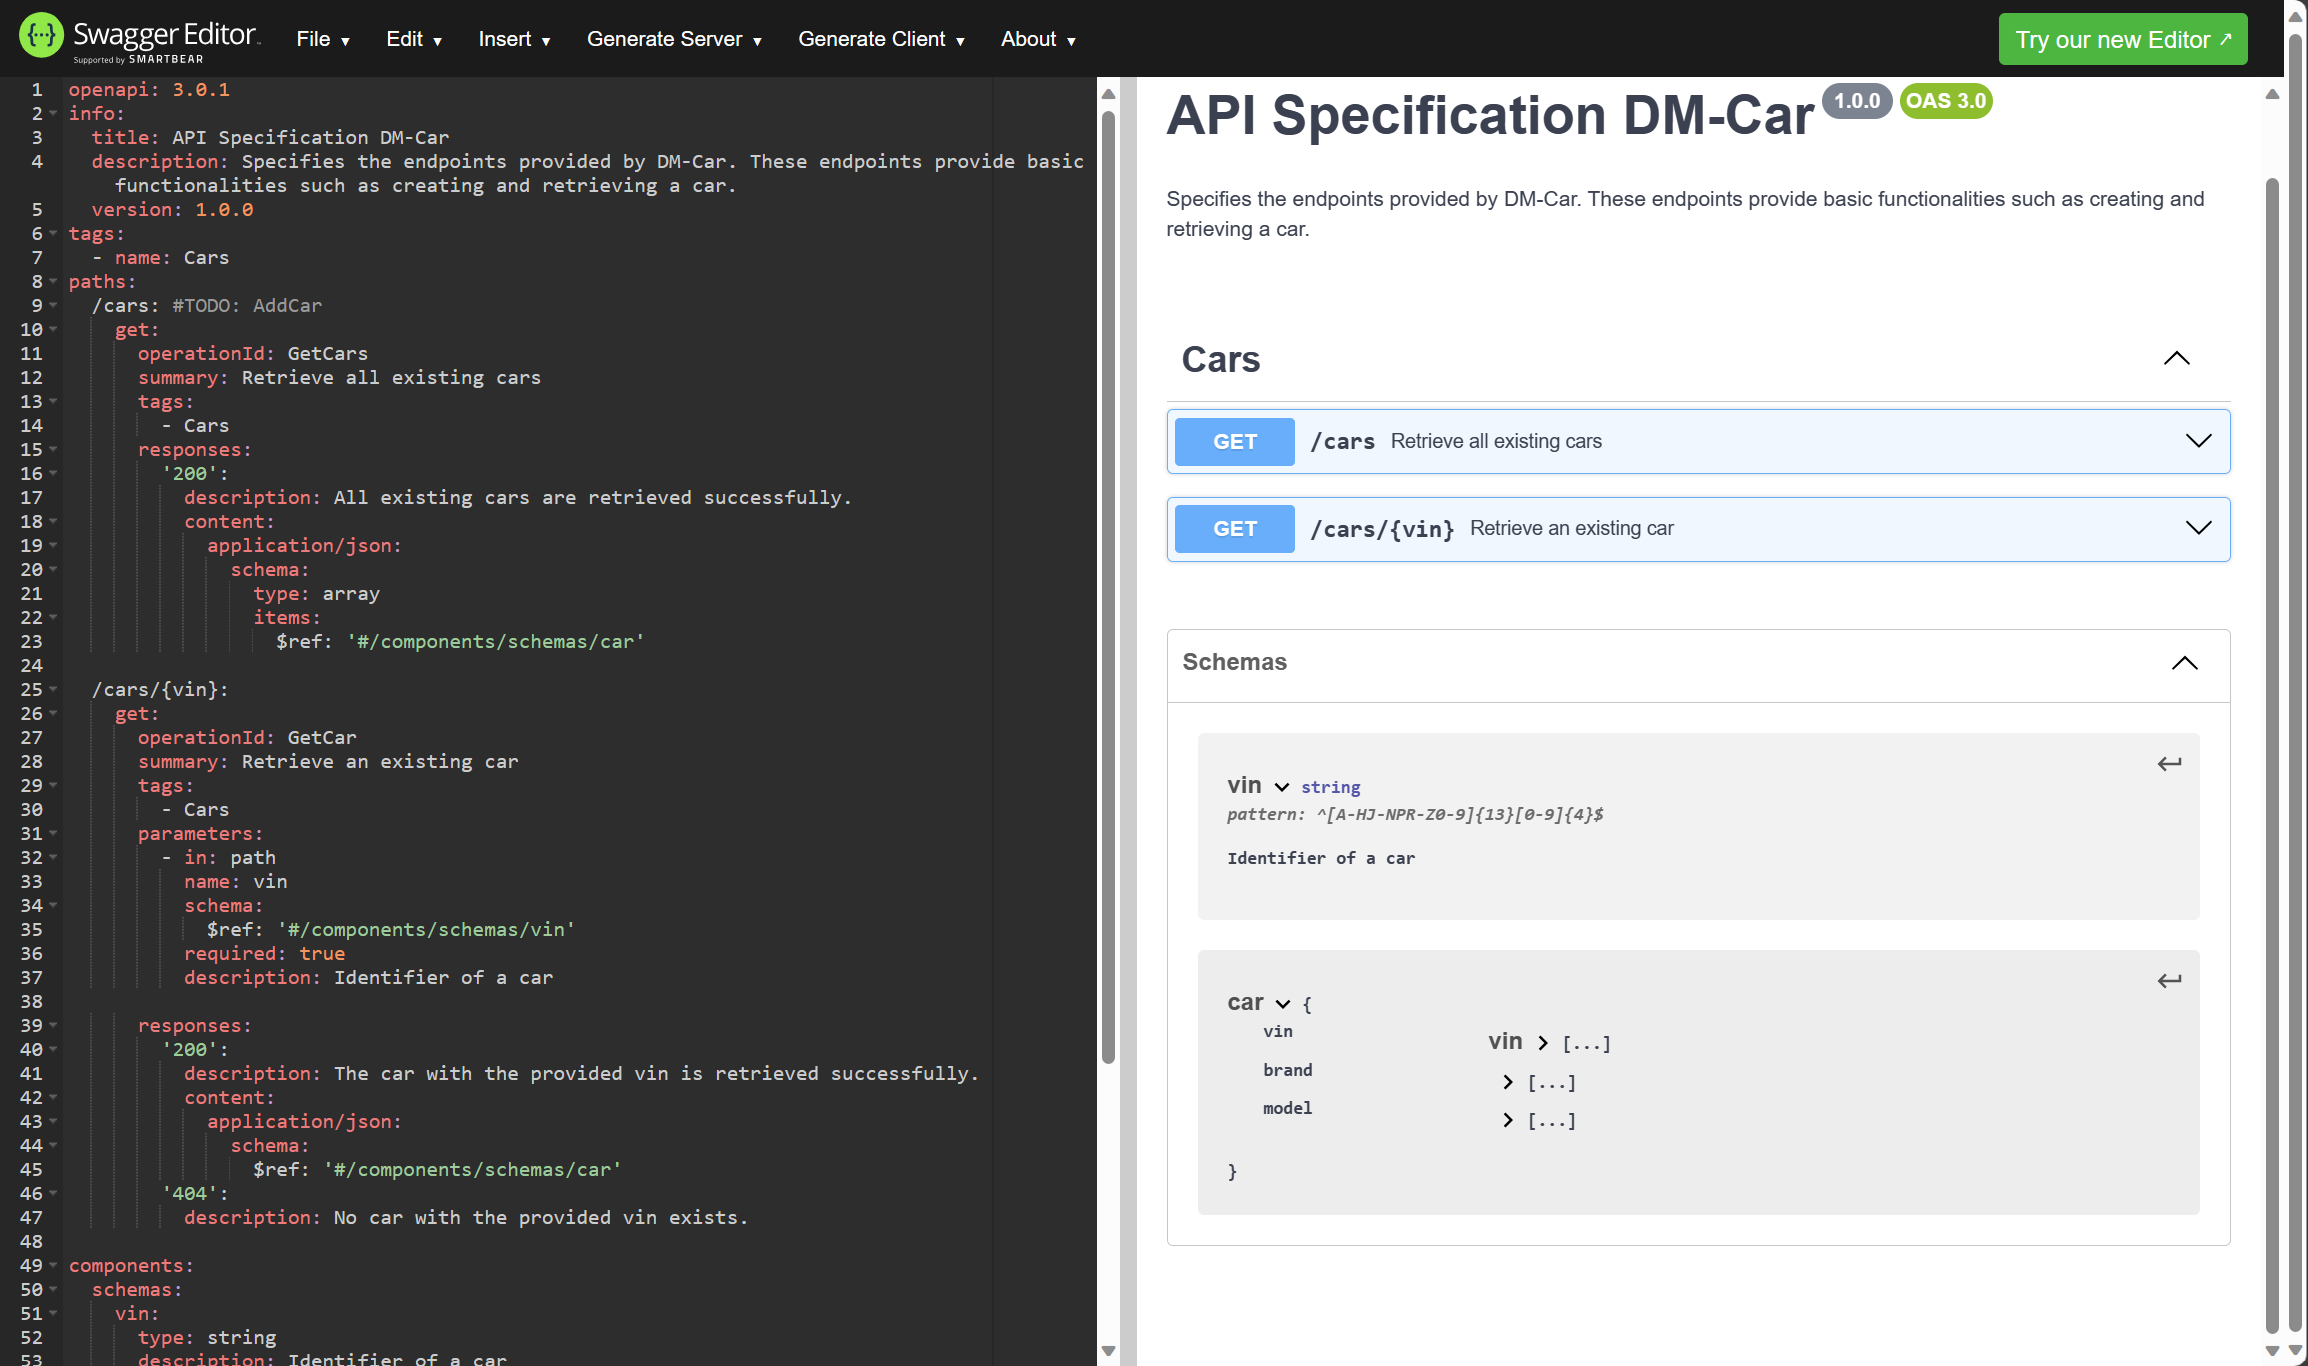
\includegraphics[width=\textwidth]{figures/microservices/dmCar/ms_dmCar_swaggerEditorUI.png}
    \caption{Swagger Editor UI}
    \label{fig:ms_dmCar_swaggerEditorUI}
\end{figure}

\subsubsection*{getCar() in OpenAPI Specification}
The lines 26 to 47 in the OpenAPI specification are relevant for the specification of the \texttt{getCar()} method.
The specification starts with the path being defined, in this case \texttt{/cras/\{vin\}}.

After that the HTTP methods are defined, here it is only the \texttt{get} method.
The specification of the method includes the operation ID, a summary, tags, parameters and the responses.
Yet, not everything is defined in this part.

The schema of the parameters and the responses are defined in the \texttt{components} section.
In this case, it is \texttt{\#/components/schemas/car}.
This part of the components defines the car object and its properties.
Due to the car being reused in multiple places, it is defined in the components section and referenced if necessary.

Therefore lines 26 to 47 define the general structure of the \texttt{getCar()} method, while the schemas are defined in \texttt{components} section, here it is lines 54 to 66.